\documentclass[a4paper]{article}

\usepackage{fontspec}
\usepackage{polyglossia}

\setmainlanguage{russian}
\setotherlanguages{english}

% download "Linux Libertine" fonts:
% http://www.linuxlibertine.org/index.php?id=91&L=1
\setmainfont{Linux Libertine O} % or Helvetica, Arial, Cambria
% why do we need \newfontfamily:
% http://tex.stackexchange.com/questions/91507/
\newfontfamily{\cyrillicfonttt}{Linux Libertine O}

\usepackage{amsmath} % Математические окружения AMS
\usepackage{amsfonts} % Шрифты AMS
\usepackage{amssymb} % Символы AMS
\usepackage{mathtext} % Русские буквы в фомулах
\usepackage{graphicx} % Вставить pdf- или png-файлы

\usepackage{xcolor}

\newcommand{\highlight}[1]{%
  \colorbox{red!50}{$\displaystyle#1$}}

\usepackage{color}
\usepackage{bbold}

\usepackage{booktabs}

\usepackage{mathrsfs} % Красивый шрифт

\usepackage{longtable}  % Длинные таблицы
\usepackage{multirow} % Слияние строкв таблице

\usepackage{indentfirst} % Отступ в первом абзаце.
\usepackage{tikz}

\newcommand*{\hm}[1]{#1\nobreak\discretionary{}%
            {\hbox{$\mathsurround=0pt #1$}}{}}

\usepackage{verbatim}

\DeclareMathOperator{\sgn}{\mathop{sgn}}
\DeclareMathOperator{\card}{\mathop{card}}
%\newcommand{\e}[1]{{\mathbb E}\left[ #1 \right]}


\usepackage{enumitem}
\usepackage{mathtools, bm, etoolbox}

\usepackage{fancyhdr}
\usepackage[margin=1in]{geometry}

\providecommand\given{}
\DeclarePairedDelimiterXPP\Aver[1]{\mathbb{E}}{[}{]}{}{
\renewcommand\given{  \nonscript\:
  \delimsize\vert
  \nonscript\:
  \mathopen{}
  \allowbreak}
#1
}




\newcommand{\shrug}[1][]{%
\begin{tikzpicture}[baseline,x=0.8\ht\strutbox,y=0.8\ht\strutbox,line width=0.125ex,#1]
\def\arm{(-2.5,0.95) to (-2,0.95) (-1.9,1) to (-1.5,0) (-1.35,0) to (-0.8,0)};
\draw \arm;
\draw[xscale=-1] \arm;
\def\headpart{(0.6,0) arc[start angle=-40, end angle=40,x radius=0.6,y radius=0.8]};
\draw \headpart;
\draw[xscale=-1] \headpart;
\def\eye{(-0.075,0.15) .. controls (0.02,0) .. (0.075,-0.15)};
\draw[shift={(-0.3,0.8)}] \eye;
\draw[shift={(0,0.85)}] \eye;
% draw mouth
\draw (-0.1,0.2) to [out=15,in=-100] (0.4,0.95);
\end{tikzpicture}}


\AddEnumerateCounter{\asbuk}{\russian@alph}{щ} % для списков с русскими буквами
\setlist[enumerate, 2]{label=\asbuk*),ref=\asbuk*}


\pagestyle{fancy} \makeatletter \fancyhead[L]{\footnotesize ICEF, 2016/17, «Mathematics for Economists»}

\makeatletter
\newcommand*{\rom}[1]{\expandafter\@slowromancap\romannumeral #1@}
\makeatother

\usepackage{wrapfig}

 \begin{document}
 \begin{center}
 {\Large{Конспект лекции 20.12.16}}
 \end{center}
  \begin{center}
 {\large{Яцушко Кирилл}}
 \end{center}

 Перед тем, как мы перейдём к выводу модели Блэка-Шоулза, рассмотрим 3 мелких сюжета. Эти сюжеты содержат промежуточные вычисления, результаты которых будут использоваться в дaльнейшем.

 \section {Три мелких сюжета}
 \subsection {Первый мелкий сюжет}
 Вычислим значение величины $\Aver{e^{\alpha x}}$, где $X \sim N(\mu;\sigma^2)$. Есть два способа решить эту задачу.
 \subsubsection{Способ первый}
 Стандартизируем нашу случайную величину:

 \begin{align*}
     \frac{x-\mu}{\sigma} &= z \sim N(0;1) \\
     x &= z \sigma + \mu
 \end{align*}


Вычислим значение матожидания "честно", с помощью интеграла:

 \begin{multline*}
     \Aver{e^{\alpha x}} = \Aver{e^{\alpha (\sigma z + \mu)}} = \Aver{e^{\alpha \sigma z + \alpha \mu}} = e^{\alpha \mu} \times \Aver{e^{\alpha \sigma z}} = e^{\alpha \mu} \times \int\limits_{-\infty}^{\infty} e^{\alpha \sigma z} f(z) dz = e^{\alpha \mu} \times \int\limits_{-\infty}^{\infty} e^{\alpha \sigma z} \frac{1}{\sqrt{2 \pi}}e^{- \frac{z^2}{2}} dz = \\ = e^{\alpha \mu} \times \int\limits_{-\infty}^{\infty} \frac{1}{\sqrt{2 \pi}} e^{-\frac{1}{2}(z^2-2 \alpha \sigma z + \alpha^2 \sigma^2)+\frac{1}{2}\alpha^2 \sigma^2} dz = e^{\alpha \mu + \frac{\alpha^2 \sigma^2}{2}} \times \int\limits_{-\infty}^{\infty} \frac{1}{\sqrt{2 \pi}} e^{-\frac{1}{2}(z-\alpha \sigma)^2} dz = \\ = (\text{введём замену } \tilde{z} = z - \alpha \sigma) = e^{\alpha \mu + \frac{\alpha^2 \sigma^2}{2}} \times \int\limits_{-\infty}^{\infty} \frac{1}{\sqrt{2 \pi}} e^{- \frac{\tilde{z}^2}{2}} d \tilde{z} = e^{\alpha \mu + \frac{\alpha^2 \sigma^2}{2}}
 \end{multline*}

 \subsubsection{Способ второй}

 Перефразируем задачу в терминах броуновского движения: необходимо вычислить $\Aver{e^{\alpha (\mu + W_{t})}}$, где $W_{t} \sim N(0;t)$, $\mu + W_{t} \sim N(\mu;t)$. Решим эту задачу в рамках небольшого упражнения. Держим в голове идею о том, что матожидание удобно считать для процессов, являющихся мартингалами.
 \vspace{5mm}

 \par {\bf\underline{Упражнение}}

 1) $Y_{t} = e^{\alpha (\mu + W_{t})}$. Найти $dY_{t}$, записать в краткой и в полной форме записи.

 2) Проверить, является ли $Y_{t}$ мартингалом.

 3) Придумать такую $f(t)$, чтобы $Z_{t} = f(t) \times Y_{t}$ был мартингалом.
 \vspace{5mm}

  \par {\bf{Решение}}

 1) $dY_{t} = \alpha e^{\alpha (\mu + W_{t})} dW_{t} + \frac{1}{2} \alpha^{2}e^{\alpha(\mu + W_{t})} dW_{t^{2}}$.

 Таким образом, краткая форма записи:

\begin{equation*}
     dY_t = \alpha e^{\alpha (\mu + W_t)} \, dW_t + \frac{1}{2} \alpha^2 e^{\alpha(\mu + W_t)} \, dt
\end{equation*}

 А в полной форме записи:

  \begin{equation*}
  Y_{t} = Y_{0} + \int\limits_{0}^{t} \alpha e^{\alpha(\mu+W_{s})} dW_{s} + \highlight{\int\limits_{0}^{t} \frac{\alpha^{2}}{2}e^{\alpha(\mu+W_{s})}ds}
  \end{equation*}

  \newpage

  2) Какие у нас есть способы проверить, что процесс является мартингалом? Первый способ — это по определению проверить, что $\Aver{Y_{t+s} \given \mathcal{{F}}_{t}} = Y_{t}$. Второй способ — это использовать свойство интеграла Ито:

    \begin{equation*}
 Y_{t} = Y_{0} + \int\limits_{0}^{t}A_{u}dW_{u} \text{— мартингал}
  \end{equation*}

  Мы видим, что не присутствуй в полной форме записи выделенная красным цветом часть, наш процесс был бы мартингалом. Но сейчас он не мартингал. \shrug

  3) $dZ_{t} = d(f(t) \times Y_{t}) = f'_t Y_t dt + f(t) dY_t + 0 \times \frac{1}{2}(dY_t)^2 = f'_t Y_t dt + f(t)(\alpha e^{\alpha (\mu + W_t)} dW_t + \frac{1}{2} \alpha^2 e^{\alpha (\mu + W_t)}dt)$

   Условие, чтобы $Z_t$ был мартингалом:

   \begin{align*}
     f'_t Y_t dt + f(t) (\frac{1}{2} \alpha^2 e^{\alpha(\mu + W_t)}dt) = 0 \\
     f'_t + f(t) \frac{\alpha^2}{2} = 0 \\
     f'_t = - f(t) \frac{\alpha^2}{2} \\
     f(t) = e^{-\frac{\alpha^2}{2}t}
 \end{align*}

  Таким образом, мы выяснили, что процесс $Z_t = e^{-\frac{\alpha^2}{2}t} \times e^{\alpha(\mu + W_t)} $ является мартингалом. Действительно: $\Aver{Z_t} = \Aver{Z_0} = e^{\alpha \mu}$. Если заменить $Z_t$ и провести небольшие преобразования, то получим: $\Aver{e^{\alpha(\mu + W_t)}}=e^{\alpha \mu + \frac{\alpha^2 t}{2}}$.

   \begin{wrapfigure}{r}{0.3\linewidth}
     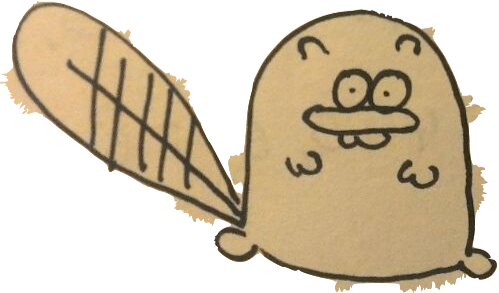
\includegraphics[width=\linewidth]{06_beaver.png}
 \end{wrapfigure} Мудрый стохастический бобр без труда заметил, что полученный нами результат совпал с результатом, который мы получили первым способом. А вы заметили?\\

  \subsection {Второй мелкий сюжет}

  Необходимо выразить с помощью $F(t)$ (функция распределения N(0;1)) $P(\sigma W_t > a)$. Делается это следующим образом:

  \begin{equation*}
  P(\sigma W_t > a) = P(\frac{W_t}{\sqrt{t}} > \frac{a}{\sigma \sqrt{t}}) = 1-P(\frac{W_t}{\sqrt{t}} \le \frac{a}{\sigma \sqrt{t}} ) = 1 - F(\frac{a}{\sigma \sqrt{t}})
  \end{equation*}

  \subsection {Третий мелкий сюжет или Теорема Гирсанова}

  Прежде чем сформулировать теорему Гирсанова, рассмотрим два упражнения.
  \vspace{5mm}

  \par {\bf\underline{Упражнение}}

  Дано распределение, заданное таблицей:
  \vspace{5mm}

\begin{tabular}{llll}
\hline
\textbf{Y}             & 0 & 1 & 2     \\ \hline
\textbf{вероятность P} & a & b & 1-a-b \\ \hline
\end{tabular}
\vspace{5mm}



1) Можно ли подобрать вероятности таким образом, чтобы $Y \sim Bin(n=2,p=\frac{1}{3})$?

2) Можно ли подобрать вероятности таким образом, чтобы $Y \sim Bin(n=4,p=\frac{1}{2})$?

\vspace{5mm}

\par {\bf{Решение}}

  1) Можно. $a = \frac{4}{9}$, $b = \frac{4}{9}$.

  2) Нельзя.

  \pagebreak

  \par {\bf\underline{Упражнение}}

   Дано распределение, заданное таблицей:

  \vspace{5mm}
\begin{tabular}{llll}
\hline
\textbf{}        & \textbf{$Y_2$ = - 2} & \textbf{$Y_2$ = 0} & \textbf{$Y_2$ = 2} \\ \hline
\textbf{$Y_1$ = -1} & a               & 0,4 - a         & 0,1             \\ \hline
\textbf{$Y_1$ = 1}  & 0,2             & b               & 0,3-b
\end{tabular}
\vspace{5mm}

Можно ли подобрать a и b так, чтобы случайный процесс $(Y_1,Y_2)$ был мартингалом? Если да, то подберите эти значения.
  \vspace{5mm}

\par {\bf{Решение}}

Заметим, что $\Aver{Y_2 \given Y_1} = Y_1$. Тогда:

\[
	\left\{
		\begin{aligned}
			&\Aver{Y_2 \given Y_1 = -1} = -1  \\
			&\Aver{Y_2 \given Y_1 = 1 } = 1   \\
		\end{aligned}
	\right.
\]


  \begin{align*}
    & P (Y_1=-1) = 0,5 \\
    &\Aver{Y_2 \given Y_1=-1} = -2 \times \frac{a}{0,5} + 0 \times \frac{0,4-a}{0,5} + 2 \times \frac{0,1}{0,5} = -1 \\
    &-2a+0,2=-0,5 \\
    &-2a=-0,7 \\
    &a=0,35 \\
    &-2 \times \frac{0,2}{0,5} + 2 \times \frac{0,3 - b}{0,5} =1 \\
    &-0,4 + 0,6 -2b =0,5\\
    &b  <0
 \end{align*}
Мы получили, что \textbf{вероятность b должна быть отрицательной}. Такого не бывает, поэтому ответ: нет, подобрать нельзя.


  \vspace{5mm}

  \par {\bf\underline{Теорема Гирсанова}}

Если $W_t$ - броуновское движение для вероятности P, то можно найти такую вероятность $\tilde{P}$, что $Y_t = W_t + \mu t$ будет броуновским движением для вероятности $\tilde{P}$.



 \section {Модель Блэк-Шоулза}

 В модели Блэк-Шоулза есть всего два актива:

 \begin{itemize}
   \item  Акции с ценой $S_t$
   \begin{itemize}
     \item  $dS_t = \mu S_t dt + \sigma S_t dW_t$
     \item  $S_t = S_0 \times e^{(\mu - \frac{\sigma^2}{2})t} + \sigma W_t$
     \end{itemize}
     \item Безрисковые облигации с ценой $B_t$
     \begin{itemize}
     \item  $dB_t=B_t \times r \times dt$
     \item  $B_t = B_0 \times e^{rt}$
     \end{itemize}
 \end{itemize}
В этой модели предполагается отсутствие арбитража, отсутствие транзакционных издержек и непрерывность количества активов.

 \vspace{5mm}

  \par {\bf\underline{Основное упражнение}}

  Инвестор сейчас находится в моменте времени $t=0$ и имеет на руках актив, за который в неслучайный момент времени T он получит $S^2_T$ рублей. Мы обозначим цену актива как $X_t$. Для этого актива можно сконструировать имплицирующий портфель, в котором будет $A_t$ акций и $\frac{X_t -A_t S_t}{B_t}$ облигаций. Стоимость такого портфеля в произвольный момент времени будет выражаться как:\\
  \[
  X_t = X_0 + \int\limits_{0}^{t}A_u d S_u + \int\limits_{0}^{t}\frac{X_u - A_u S_u}{B_u}dB_u\]

  Нашей задачей является поиск справедливой цены $X_0$ в начальный момент времени.


   \vspace{5mm}

  \par {\bf\underline{Упражнение}}

  В этом упражнении мы изучим, как изменяется во времени цена имплицирующего портфеля. Нужно найти:

  1) $dX_t$ — ?

  2) $d(e^{-rt}X_t)$ — ?

  \vspace{5mm}

\par {\bf{Решение}}

\[
dX_t = A_t d S_t + \frac{X_t-A_t S_t}{B_t} dB_t = A_t d S_t + (X_t - A_t S_t)rdt \]

\begin{multline*}
d(e^{-rt}X_t) = e^{-rt} d X_t - rX_t e^{-rt}dt = e^{-rt}(A_t d S_t +(X_t - A_t S_t)rdt - rX_tdt) = e^{-rt} (A_t d S_t - A_t S_t rdt) = \\ = A_t e^{-rt} (\mu S_t dt + \sigma S_t d W_t - S_t r dt) = S_t A_t e^{-rt} (\mu dt + \sigma d W_t - rdt) = S_t A_t e^{-rt} ((\mu - r) dt + \sigma d W_t)
\end{multline*}


  Заметим, что процесс $Y_t = e^{-rt}X_t$ не является мартингалом. Воспользуемся теоремой Гирсанова.

  \[
dY_t = e^{-rt} S_t A_t \sigma (\frac{\mu -r}{\sigma} dt + dW) \]


  Рассмотрим выражение в скобках.

  \[
d \tilde{W} = \frac{\mu-r}{\sigma}dt + dW \]

  \[
\tilde{W_t} = \tilde{W_0} + \int\limits_{0}^{t}\frac{\mu-r}{\sigma}du + \int\limits_{0}^{t}dW_u\]

  \[ \tilde{W_t} = \tilde{W_0} + \frac{\mu-r}{\sigma}t + W_t
 \]

 Вопрос в следующем: является ли процесс $\tilde{W_t}$ броуновским движением? Вообще говоря, нет. Но теорема Гирсанова говорит, что найдется такая вероятность $\tilde{P}$, что он будет броуновским движением. Тогда относительно вероятности $\tilde{P}$ процесс $dY_t = e^{-rt} S_t A_t \sigma d \tilde {W_t}$ будет являться броуновским движением. Таким образом, мы доказали, что:
  \begin{equation*}
  \forall t X_0 = \Aver{e^{-rt} X_t \given \mathcal{F}_0}_{\tilde{P}}
  \end{equation*}

  Пользуясь этим фактом, мы без труда ответим на изначально поставленный вопрос:

  \begin{multline*}
X_0 = \Aver{e^{-rT} X_T \given \mathcal{F}_0}_{\tilde{P}} = e^{-rT} \Aver{S^2_{t} \given \mathcal{F}_0} = e^{-rT} \times \Aver{S^2_0 e^{2(\mu - \frac{\sigma^2}{2})T}+2\sigma W_T \given \mathcal{F}_0} = \\ = e^{-rT} S^2_0 e^{2(\mu - \frac{\sigma^2}{2})T} \Aver{e^{2\sigma(\tilde{W_T}-\frac{\mu-r}{\sigma}T)}\given \mathcal{F}_0} = e^{-rT} S^2_0 e^{2\mu T - \sigma^2 T} e^{-2(\mu - r)T} \Aver{e^{2 \sigma \tilde{W_t}} \given \mathcal{F}_0} = \\ = e^{rt} S^2_0 e^{- \sigma^2 T} \Aver{e^{2 \sigma \tilde{W_T}}} = S^2_0 e^{rT-\sigma^2T} e^{2\sigma \times 0 + \frac{4\sigma^2 T}{2}} =  S^2_0e^{rT+\sigma^2T} = X_0 
\end{multline*}
\end{document}
